% !TeX root = ../main.tex
% NOTA: los cambios aparecen en azul. Requiere \usepackage{xcolor} en el preámbulo.
\chapter{Del problema a la solución: contexto y propuesta}
\label{cap:problema-solucion}
Este capítulo concreta el punto de partida, qué problema se quiere resolver y qué solución se propone para hacerlo, apoyándose en el análisis del sector y de los productos existentes que se desarrolla en el estado del arte (capítulo~\ref{cap:estado-arte}). En primer lugar se resume el contexto y se concreta el problema (sección~\ref{sec:contexto}). A continuación se presenta la propuesta, el ecosistema VH SimGrid, formado por tres periféricos y una aplicación de escritorio que los integra (sección~\ref{sec:propuesta}). Por último, se estudia la viabilidad de la propuesta desde los puntos de vista estratégico, de negocio, de riesgos y económico (sección~\ref{sec:viabilidad}).

\section{Contexto}
\label{sec:contexto}
El simracing ha pasado en poco más de una década de ser una afición minoritaria a convertirse en un mercado consolidado, con competiciones oficiales, equipos profesionales y cientos de miles de aficionados que compiten desde casa (sección~\ref{sec:simracing-entrenamiento}). Ese crecimiento se ha apoyado en la llegada al consumidor de tecnologías que antes eran exclusivas de la gama profesional, como las bases \textit{direct drive} o las pedaleras con célula de carga (sección~\ref{sec:fundamentos-tecnicos}). Sin embargo, el acceso a un equipo de simulación de calidad sigue encontrando tres obstáculos, que constituyen el problema que plantea este trabajo: los periféricos son caros, son cerrados y no existe un software que los una.

\paragraph{Periféricos caros.}
El periférico es el componente que más pesa en el coste de un equipo de simracing. Una base \textit{direct drive} de par medio se sitúa entre los 500 y los 850~euros: la Moza R12~V2, de 12~N\,m, tiene un precio oficial de 529~euros; la Fanatec ClubSport~DD, de 15~N\,m, de unos 600~euros, y la Simagic Alpha EVO Pro, de 18~N\,m, salió al mercado por 839~euros \parencite{moza_web, fanatec_web, bsimracing_2025_alpha_evo}. A la base hay que sumar el aro y la pedalera, que no son accesorios menores: un aro de tipo GT de gama media y una pedalera con célula de carga de dos pedales cuestan cada uno en torno a 400--450~euros en el catálogo del mismo fabricante \parencite{moza_web}. Un puesto completo de gama media supera así con facilidad los 1.200~euros, sin contar el \textit{cockpit} ni el ordenador. Como se detalla en el estado del arte, buena parte de ese precio no se explica por la tecnología, que se basa en componentes disponibles a bajo coste gracias a la robótica y a la movilidad eléctrica, sino por la marca, las licencias y los márgenes de un mercado dominado por pocos fabricantes (sección~\ref{sec:soluciones-comerciales}).

\paragraph{Periféricos cerrados.}
Cada fabricante construye su propio ecosistema y lo protege. El aro se une a la base mediante un anclaje rápido propietario, de modo que un aro de una marca no se puede montar en la base de otra sin un adaptador. El firmware y los protocolos de comunicación no son públicos: el usuario no puede saber cómo se calcula el \textit{force feedback} ni modificar su comportamiento más allá de los parámetros que el fabricante decide exponer. Esta dependencia tiene además un riesgo para el comprador, que queda ligado a la continuidad de la marca. El caso de Fanatec, cuya empresa matriz entró en concurso de acreedores en 2024 y acabó adquirida por Corsair \parencite{businesswire_2024_corsair_fanatec}, mostró que incluso el fabricante líder puede atravesar dificultades que ponen en duda el soporte de los productos ya vendidos (sección~\ref{sec:soluciones-comerciales}). Los proyectos abiertos DIY ofrecen una alternativa a este modelo, pero suelen centrarse en un único periférico y exigen al usuario conocimientos técnicos para montar y configurar el conjunto.

\paragraph{Sin un software que los una.}
El tercer obstáculo aparece una vez que el equipo está montado. Cada fabricante distribuye su propia aplicación de configuración, como Moza Pit House, Fanatec App o SimPro Manager, y un usuario que combina periféricos de varias marcas tiene que instalar y utilizar software de diferentes distribuidores. A ellas se suman las herramientas de apoyo al piloto como SimHub para las pantallas, los LEDs y la vibración, Crew Chief como ingeniero por voz y una o varias aplicaciones de análisis de telemetría (sección~\ref{sec:software-apoyo}). Cada programa tiene su instalación, sus perfiles y su forma de leer los datos del simulador, y ninguno conoce el hardware sobre el que se ejecuta: la herramienta que enciende los LEDs del aro no puede ajustar el \textit{force feedback} de la base ni la curva del freno. El resultado es un puesto fragmentado donde el usuario final tiene que configurar todo evitando problemas de compatibilidad, lo que puede llegar a ser frustrante y complicado para aquellos que no tienen experiencia.

\paragraph{Planteamiento del problema.}
De los tres obstáculos anteriores se deriva el problema que aborda este trabajo: no existe un sistema que ofrezca un puesto de simracing completo, con prestaciones de gama media y a un coste sensiblemente inferior al de los equipos comerciales, cuyos periféricos y cuyo software se hayan diseñado juntos. Resolverlo exige actuar a la vez sobre el hardware y sobre el software. En el hardware, creando periféricos propios a partir de componentes accesibles, sin depender del ecosistema de ningún fabricante. En el software, desarrollando una aplicación específica para esos periféricos, que los configure en vivo sin necesidad de reprogramarlos, de modo que resulte accesible para la mayor parte del público, que no tiene conocimientos de electrónica ni sabe grabar un firmware, y que reúna además las funciones que hoy se reparten entre programas independientes, como las pantallas de datos, el ingeniero por voz, la estrategia de carrera y el análisis de telemetría. Este es el planteamiento del sistema que se propone en la sección siguiente.


\section{Propuesta de valor}
\label{sec:propuesta}

Para resolver el problema planteado se propone desarrollar VH SimGrid, un ecosistema de simracing formado por tres periféricos de fabricación propia y una aplicación de escritorio diseñada específicamente para ellos. Los periféricos cubrirán los tres elementos básicos de un puesto de simulación: una base con \textit{force feedback}, la VH Grid DD15; una pedalera, la VH Axis, y un aro, el VH Formula Apex. La aplicación, que da nombre al conjunto, se encargará de configurarlos y reunirá además las funciones de apoyo al piloto que hoy se reparten entre programas independientes. La tabla~\ref{tab:ecosistema} resume el papel de cada componente.

\begin{table}[htbp]
	\centering
	\caption{Componentes del ecosistema VH SimGrid propuesto.}
	\label{tab:ecosistema}
	\small
	\begin{tabular}{|l|p{0.36\textwidth}|p{0.3\textwidth}|}
		\hline
		\textbf{Componente} & \textbf{Función} & \textbf{Enfoque} \\
		\hline
		VH Grid DD15 & Base con \textit{force feedback} que transmite al piloto las fuerzas de la dirección & Motor sin escobillas de bajo coste y controladora FOC con firmware propio \\
		\hline
		VH Axis & Pedalera de acelerador, freno y embrague & Sensores de posición y célula de carga en el freno \\
		\hline
		VH Formula Apex & Aro de tipo Fórmula con mandos e indicadores luminosos & Microcontrolador, matriz de botones y LEDs \\
		\hline
		VH SimGrid & Configuración de los periféricos y apoyo al piloto en un único programa & Aplicación de escritorio para Windows \\
		\hline
	\end{tabular}
\end{table}

El planteamiento responde directamente a los tres obstáculos identificados en la sección~\ref{sec:contexto}. Frente al coste, los periféricos se construirán con componentes de bajo precio procedentes de la robótica, la movilidad eléctrica y la electrónica de aficionado, que funcionan según los mismos principios que los periféricos comerciales. Frente a los ecosistemas cerrados, todos los periféricos se presentarán al ordenador como dispositivos USB estándar, de modo que cualquier simulador pueda usarlos sin controladores específicos. Frente a la fragmentación del software, los periféricos y la aplicación se diseñarán juntos, para que la aplicación conozca cada dispositivo y pueda ajustarlo, y reúna en un solo programa la configuración y las herramientas de apoyo al piloto.

A estos tres criterios se suma un cuarto: que el sistema pueda usarlo alguien sin conocimientos técnicos. Una vez montados los periféricos, el usuario no debería tener que programar ni grabar firmware para configurarlos. Los ajustes se harán desde la aplicación y se aplicarán en vivo, y las actualizaciones de firmware se instalarán también desde ella, con la menor intervención posible. Las subsecciones siguientes describen la propuesta para cada componente.

\subsection{Base de \textit{force feedback}}
\label{sec:propuesta-base}

La base, que recibirá el nombre de VH Grid DD15, es el periférico que más influye en la experiencia de conducción y también el más caro, por lo que es el componente central de la propuesta. Su objetivo es ofrecer un \textit{force feedback} comparable al de las bases \textit{direct drive} de gama media del mercado con un coste muy inferior.

\paragraph{Enfoque.}
Se adoptará la arquitectura \textit{direct drive}, en la que el aro se monta directamente sobre el eje del motor, porque es la única que transmite la señal del simulador sin las holguras, la elasticidad y el rozamiento de una transmisión por engranajes o por correa (véase la sección~\ref{sec:bases-ffb}). La dificultad de esta arquitectura no está en la mecánica, sino en el motor y en su control. Para el motor se plantea reutilizar un motor de buje sin escobillas de los que se fabrican en grandes series para vehículos de movilidad personal como patinetes eléctricos, que por su construcción dan mucho par a baja velocidad y cuestan una fracción de un servomotor específico. Para el control se partirá de una controladora de código abierto con control vectorial (FOC), sobre la que se desarrollará un firmware propio que la convierta en una base de \textit{force feedback}.

\paragraph{Funciones previstas.}
La base deberá presentarse ante el sistema operativo como un volante de \textit{force feedback} estándar mediante la clase HID PID, la extensión del estándar USB para dispositivos que generan fuerzas, de modo que los simuladores la reconozcan sin controladores y le envíen sus efectos a través de la interfaz DirectInput de Windows (véase la sección~\ref{sec:fundamentos-tecnicos}). Entre la consigna del simulador y el par del motor, el firmware aplicará una cadena de procesado ajustable desde la aplicación de los que cuenta el rango de giro, la fuerza máxima, una curva de respuesta, un filtrado por frecuencias que permita realzar o atenuar distintos tipos de efecto y perfiles que se carguen según el simulador o el tipo de coche. Además, deberá compensar el \textit{cogging} propio de los motores de buje, que de otro modo se notaría como pequeños saltos al girar el volante.

\paragraph{Seguridad.}
Una base \textit{direct drive} puede generar un par capaz de lesionar las manos o las muñecas del piloto, especialmente en un choque o si el volante se suelta a alta velocidad. Por ello, la seguridad se considera un requisito de diseño y no un añadido: el firmware deberá limitar el par y la velocidad, proteger el motor frente al sobrecalentamiento y frenar el volante en los límites establecidos, con independencia de lo que pida el simulador.



\subsection{Pedalera}
\label{sec:propuesta-pedalera}

La pedalera, que recibirá el nombre de VH Axis, recogerá las órdenes del piloto sobre el acelerador, el freno y el embrague. Después de la base, es el periférico que más influye en la consistencia del piloto, porque de ella depende que pueda repetir una frenada vuelta tras vuelta. Su objetivo es ofrecer las prestaciones de una pedalera de gama media, con freno por célula de carga y los otros dos mediante recorrido usando sensores Hall, a un coste muy inferior al de los modelos comerciales equivalentes.

\paragraph{Enfoque.}
La decisión de diseño más importante es qué magnitud mide cada pedal. En un coche real, el pedal de freno apenas se desplaza y el piloto dosifica la frenada con la presión del pie, mientras que el acelerador y el embrague se controlan por su posición (véase la sección~\ref{sec:pedaleras}). Por ello se plantea una solución mixta. El freno medirá la fuerza mediante una célula de carga, un sensor que produce una señal proporcional a la fuerza aplicada. El acelerador y el embrague medirán su recorrido con sensores de efecto Hall, que detectan la posición de un imán sin contacto físico y, por tanto, no se desgastan ni generan el ruido de los potenciómetros que montan las pedaleras de gama de entrada. La estructura y los pedales serán de fabricación propia, con elementos elásticos que den al freno una resistencia progresiva, y un microcontrolador leerá los tres sensores y se comunicará con el ordenador.

\paragraph{Funciones previstas.}
La pedalera se presentará ante el sistema operativo como un mando USB estándar con tres ejes, por lo que cualquier simulador podrá usarla sin controladores. El microcontrolador leerá los sensores a una frecuencia elevada y filtrará su ruido, de modo que la señal llegue al simulador estable y sin retraso apreciable. Desde la aplicación, el usuario podrá calibrar cada pedal de forma guiada, indicando su posición de reposo y su máximo recorrido, y en el caso del freno, la fuerza máxima en kilogramos que desea aplicar. También podrá ajustar la curva de respuesta de cada pedal, que modifica la relación entre el pie del piloto y el valor que recibe el simulador, así como las zonas muertas al principio y al final del recorrido. Estos ajustes se guardarán en la memoria de la propia pedalera, de modo que se conserven aunque se conecte a otro ordenador o la aplicación no esté abierta.

\subsection{Aro}
\label{sec:propuesta-aro}

El aro, que recibirá el nombre de VH Formula Apex, es la parte del volante que el piloto sujeta y desde la que maneja los mandos del coche sin soltar las manos. En los periféricos comerciales es también el componente en el que el precio depende menos de la tecnología siendo su electrónica sencilla, y las réplicas de volantes reales alcanzan precios superiores al de una base completa por sus licencias y sus materiales (véase la sección~\ref{sec:soluciones-comerciales}). Su objetivo es ofrecer un aro de tipo Fórmula, con los mandos y los indicadores de un volante de competición actual, fabricado con medios propios.

\paragraph{Enfoque.}
Se plantea un aro de tipo Fórmula, de pequeño diámetro y con los mandos concentrados en su parte central, que toma como referencia el volante del Aston Martin AMR23, el monoplaza con el que Fernando Alonso disputó la temporada 2023 del Campeonato del Mundo de Fórmula~1. El cuerpo del aro será de fabricación propia mediante impresión 3D, un proceso que permite iterar el diseño con rapidez y ajustar la forma de las empuñaduras y la posición de cada mando. Un microcontrolador leerá todos los mandos y gobernará los indicadores luminosos. Para leer un número elevado de pulsadores con pocos pines se empleará una matriz de botones, y los selectores rotativos se resolverán con \textit{encoders}. El aro se unirá a la base mediante un anclaje mecánico y tendrá su propia conexión con el ordenador, de modo que no dependa de un conector propietario y pueda montarse sobre otras bases.

\paragraph{Funciones previstas.}
El aro incluirá pulsadores, \textit{encoders}, levas de cambio y levas de embrague, que el ordenador reconocerá como los botones y ejes de un mando USB estándar, por lo que cualquier simulador podrá asignarlos sin controladores. Las levas de embrague podrán funcionar como un embrague convencional o con un punto de mordida ajustable, para facilitar las salidas. En la parte superior, una tira de LEDs mostrará las revoluciones del motor y avisará de los eventos de la carrera, como las banderas, la actuación de ayudas electrónicas del vehículo, el limitador de velocidad en el \textit{pit lane} o la presencia de otros coches cerca. En el centro del aro, como en los volantes de Fórmula~1, una pantalla mostrará al piloto la información de la carrera como la marcha engranada, las revoluciones, el tiempo por vuelta y la diferencia con la vuelta de referencia, el combustible o el estado de los neumáticos. Su contenido lo generará la aplicación a partir de la telemetría del simulador, podrá organizarse en varias páginas que el piloto pase con los botones del aro y se diseñará con el mismo editor que las pantallas de datos de la aplicación (véase la sección~\ref{sec:propuesta-app}). Todo ello se configurará desde la aplicación, pudiendo elegir qué efecto se muestra en cada LED, con qué colores y con qué estilo, el umbral de revoluciones de cada luz y el brillo, con perfiles que se carguen según el simulador y el coche. Como en el resto de periféricos, los ajustes básicos se guardarán en el propio aro para que funcione aunque la aplicación no esté abierta.

\subsection{Aplicación de escritorio}
\label{sec:propuesta-app}

La aplicación de escritorio, que da nombre al ecosistema, VH SimGrid, es la pieza que une los periféricos y la que responde al tercer obstáculo identificado en la sección~\ref{sec:contexto}: la falta de un software que los integre. Su objetivo es que el piloto pueda configurar todo su puesto y disponer de las herramientas de apoyo que necesita desde un único programa, sin conocimientos técnicos y sin tener que instalar y coordinar aplicaciones de distintos fabricantes.

\paragraph{Enfoque.}
Se plantea una aplicación de escritorio para Windows, el sistema operativo en el que se ejecutan la mayoría de los simuladores de PC, organizada en páginas y utilizadas una para cada periférico y una para cada herramienta de apoyo. La aplicación tendrá dos fuentes de información. Por un lado, se comunicará con los periféricos para leer su estado y enviarles los ajustes. Por otro, leerá la telemetría que publica cada simulador, es decir, los datos del coche y de la carrera en cada instante. Como cada simulador publica esos datos en su propio formato (véase la sección~\ref{sec:software-apoyo}), la aplicación incluirá una capa que los traduzca a un formato común, de modo que el resto de funciones trabajen igual con cualquier simulador compatible. Toda la información se procesará en el propio equipo del usuario, sin enviar datos a servicios externos.

\paragraph{Configuración de los periféricos.}
La aplicación detectará los periféricos al conectarlos y mostrará su estado en una pantalla de inicio, junto con los simuladores instalados. La primera vez, un asistente guiará al usuario en la configuración de cada periférico y de la telemetría de sus juegos. Desde ella se ajustarán el \textit{force feedback} de la base, la calibración y las curvas de los pedales y las luces del aro, como se ha descrito en las subsecciones anteriores. Los cambios se aplicarán en vivo y se agruparán en perfiles que podrán cargarse automáticamente al detectar el simulador o el coche en uso. La aplicación se encargará también de actualizar el firmware de los periféricos cuando haya una versión nueva, de modo que el usuario no tenga que usar herramientas de programación.

\paragraph{Pantallas de datos.}
La aplicación incluirá un \textit{dash}, una pantalla de datos como la de un coche de competición, que mostrará en la pantalla central del aro o en un monitor secundario información como la marcha, las revoluciones, los tiempos por vuelta, el estado de los neumáticos o el combustible. Se ofrecerá una colección de diseños de serie para distintos tipos de coche y un editor con el que el usuario pueda crear los suyos o modificar los existentes a partir de elementos como textos, indicadores, barras o gráficas.

\paragraph{Ingeniero de pista por voz.}
La aplicación incorporará un ingeniero de pista virtual que informará al piloto por voz durante la carrera, como haría el ingeniero de un equipo real por la radio: avisos de coches cerca, consumo de combustible, estado de los neumáticos, ritmo, diferencias con los rivales o momento de entrar a boxes. El piloto podrá también preguntarle por voz, pulsando un botón del aro asignado, sin soltar el volante. Para preparar las carreras largas, la aplicación incluirá además una calculadora de estrategia que compare distintas opciones de paradas según el reglamento de cada carrera, y la estrategia elegida será la que siga el ingeniero durante la prueba. Tanto la síntesis de voz como el reconocimiento de lo que dice el piloto funcionarán en el propio equipo.

\paragraph{Análisis de telemetría.}
Por último, la aplicación grabará automáticamente cada sesión y permitirá analizarla después, al estilo de las herramientas de análisis de datos del automovilismo profesional. El piloto podrá comparar sus vueltas con una de referencia y estudiar, canal a canal y curva a curva, la velocidad, el uso de los pedales, el giro del volante, el comportamiento de los neumáticos o la suspensión, para encontrar dónde pierde tiempo y cómo mejorar su conducción.

\section{Estudio de viabilidad}
\label{sec:viabilidad}

Antes de comenzar el desarrollo conviene comprobar que la propuesta es viable, es decir, que tiene sentido frente a las alternativas existentes, que puede llevarse a cabo con los medios disponibles y que los riesgos que implica son asumibles. Aunque este trabajo es un proyecto académico, la propuesta se analiza como si fuera un producto, porque solo así puede valorarse si resuelve de verdad el problema planteado para un usuario real. El estudio se aborda desde cuatro puntos de vista complementarios: la posición estratégica de la propuesta frente al mercado, mediante un análisis DAFO (sección~\ref{sec:dafo}); su modelo de negocio, mediante un Lean Canvas (sección~\ref{sec:lean-canvas}); los riesgos del proyecto y su plan de mitigación (sección~\ref{sec:riesgos}), y su viabilidad económica, {\color{blue}mediante el análisis de los recursos disponibles y un presupuesto estimado} (sección~\ref{sec:viabilidad-economica}).

\subsection{Análisis DAFO}
\label{sec:dafo}

El análisis DAFO es una herramienta de planificación estratégica que examina una propuesta desde dos dimensiones. En la dimensión interna se recogen las debilidades y las fortalezas, que dependen del propio proyecto y de las decisiones que se tomen en él. En la dimensión externa se recogen las amenazas y las oportunidades, que proceden del mercado y del entorno y que el proyecto no puede controlar, pero sí aprovechar o prevenir \parencite{weihrich_1982_tows}. La figura~\ref{fig:dafo} resume el análisis de VH SimGrid, que se comenta a continuación.

\begin{figure}[H]
	\centering
	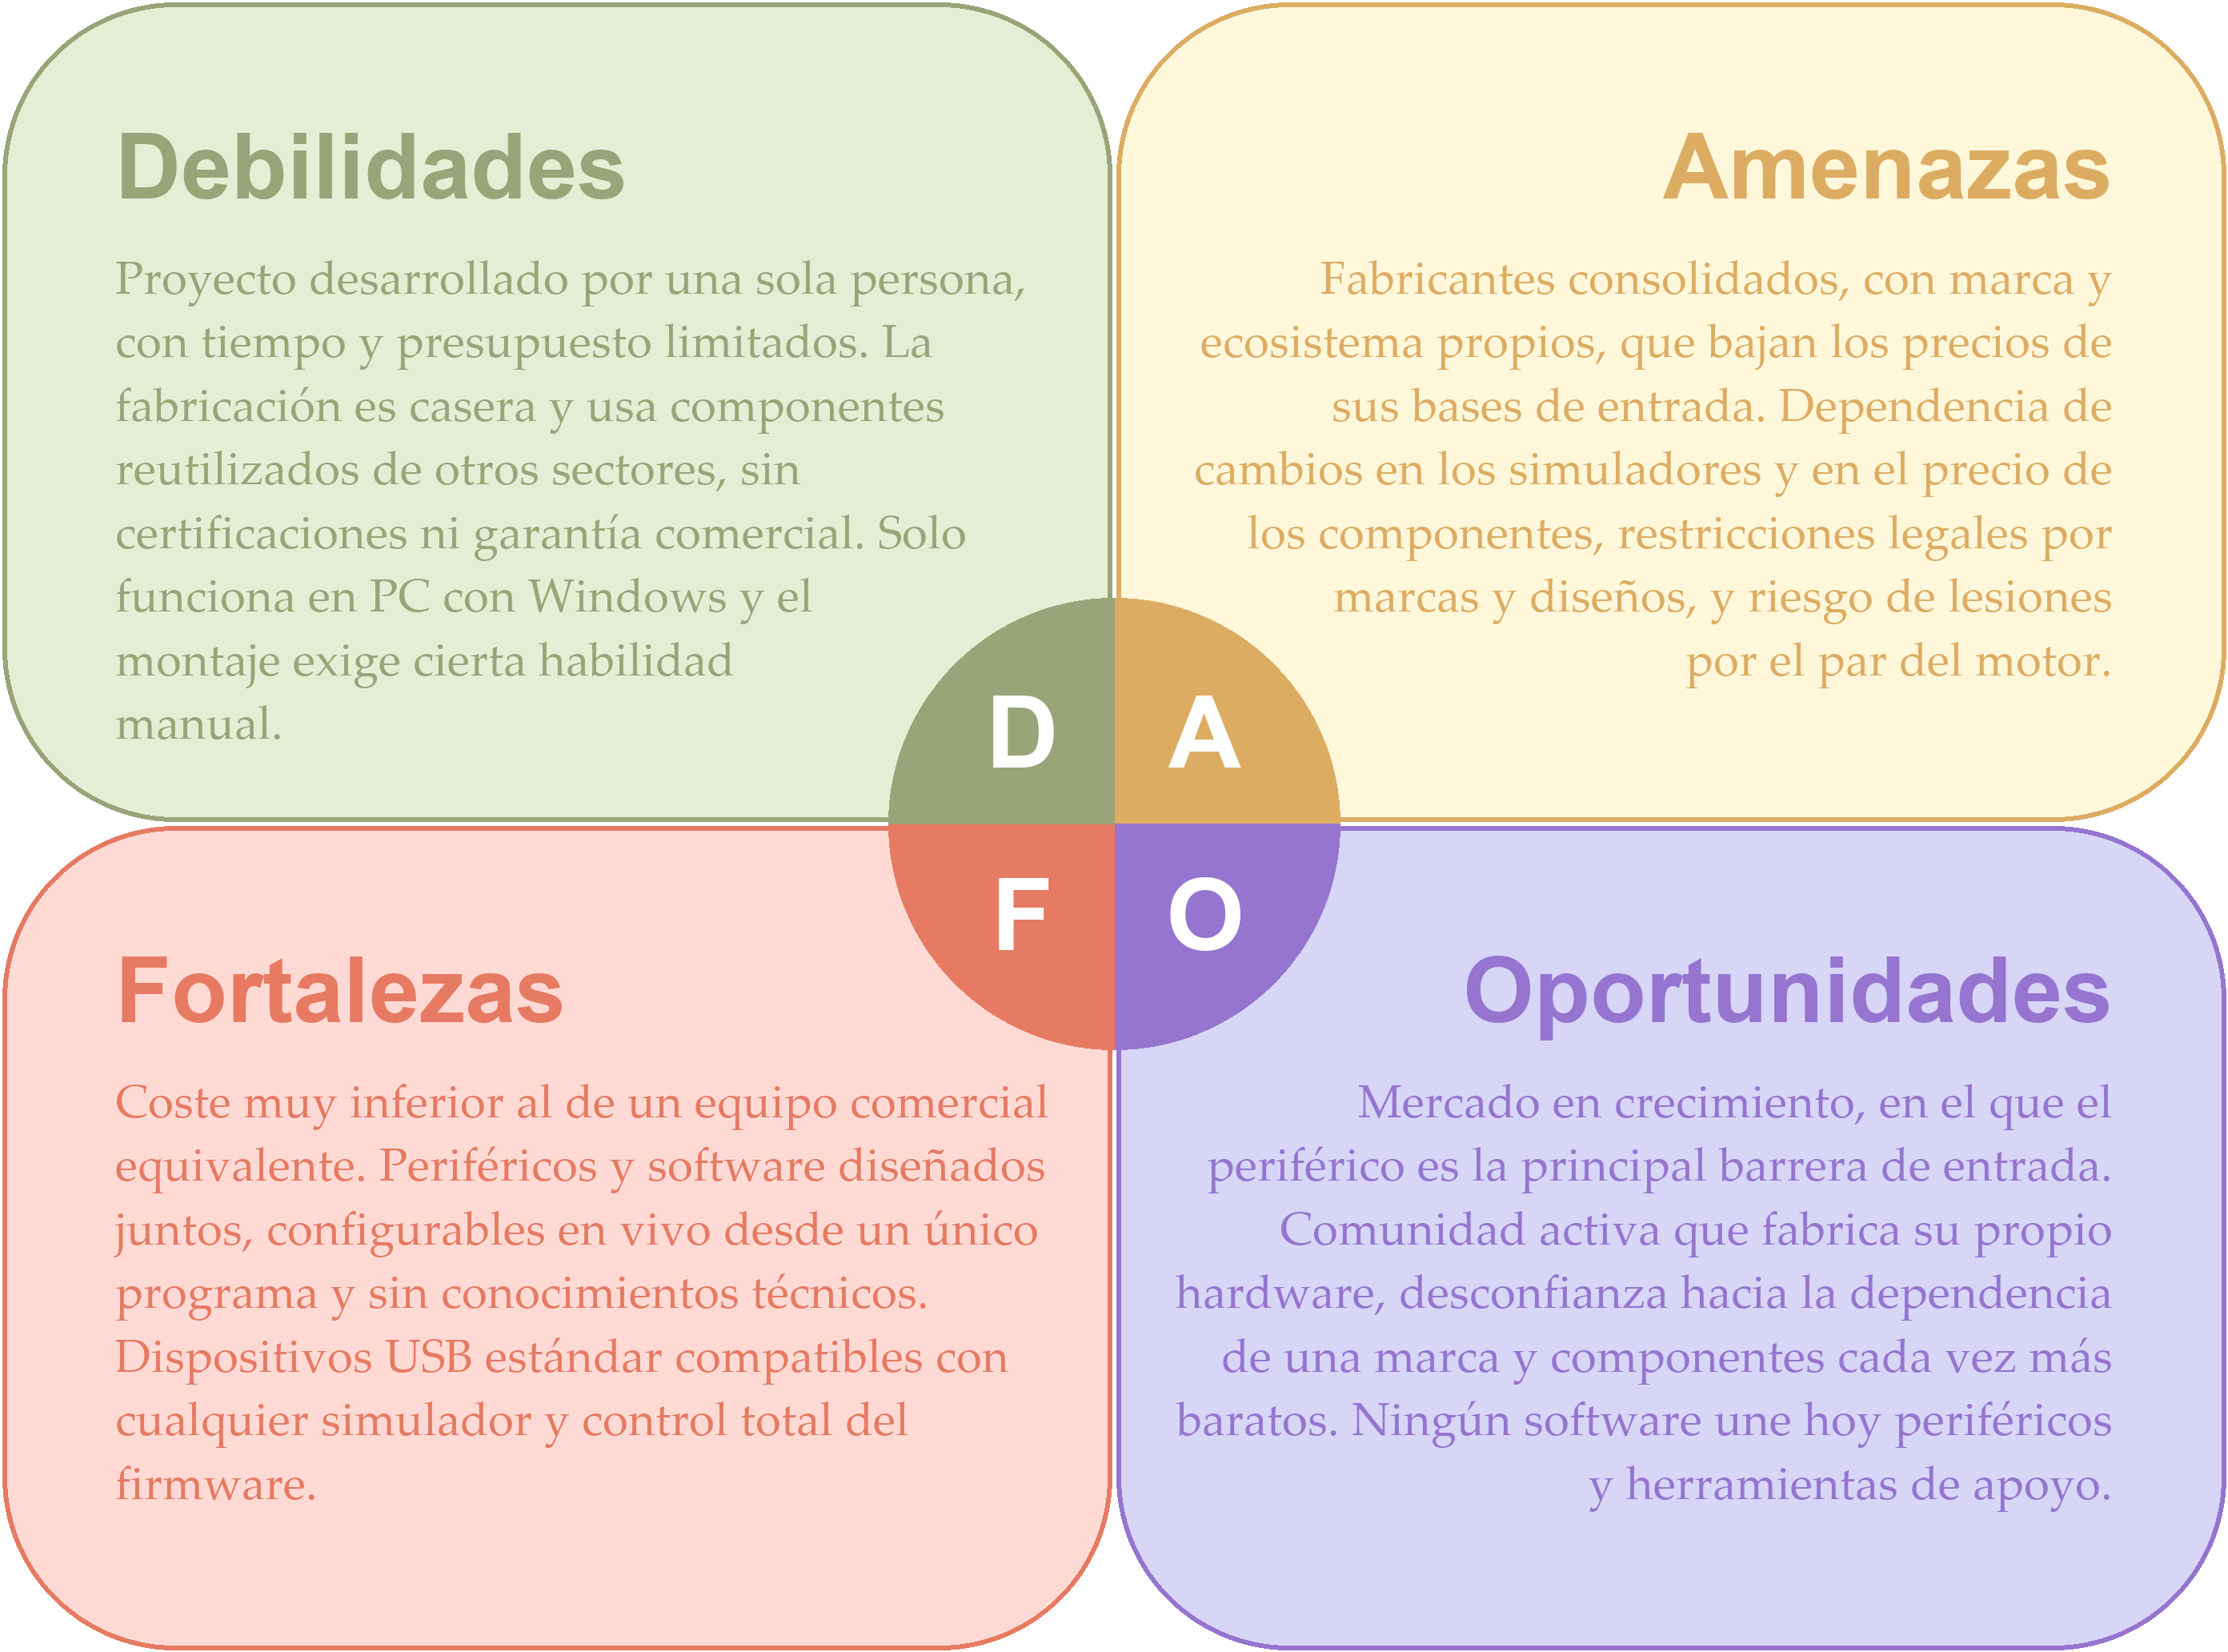
\includegraphics[width=\textwidth]{img/DAFO.png}
	\caption[Análisis DAFO del ecosistema VH SimGrid]{Análisis DAFO del ecosistema VH SimGrid. (Fuente propia)}
	\label{fig:dafo}
\end{figure}

\paragraph{Debilidades.}
La principal debilidad del proyecto es su escala. Lo desarrolla una sola persona, con un tiempo y un presupuesto limitados, frente a fabricantes con equipos de ingeniería completos. La fabricación casera, basada en la impresión 3D y en piezas mecanizadas a mano, no alcanza el acabado ni, previsiblemente, la durabilidad de un producto industrial, y los componentes clave, como el motor de la base, se reutilizan de otros sectores y no se han diseñado para esta aplicación. El sistema tampoco contará con certificaciones ni con la garantía de un producto comercial. Por último, la propuesta se limita al PC con Windows, mientras que una parte del mercado juega en consolas, y montar los periféricos exige cierta habilidad manual, aunque su configuración posterior no requiera conocimientos técnicos.

\paragraph{Amenazas.}
El mercado de periféricos evoluciona rápido. Los fabricantes han ido bajando el precio de sus bases \textit{direct drive} de entrada, que en algunos casos ya se sitúa en torno a los 330~euros \parencite{fanatec_web}, y cuentan con una marca reconocida, una comunidad de usuarios y ecosistemas completos de productos compatibles. El proyecto depende además de factores externos: los simuladores pueden cambiar el formato de su telemetría, el sistema operativo puede modificar la forma en que gestiona los dispositivos de \textit{force feedback}, y el precio y la disponibilidad de los componentes electrónicos pueden variar, como ocurrió durante la escasez de chips de 2021 \parencite{endor_web}. Tomar como referencia el volante de un monoplaza real plantea restricciones de propiedad intelectual sobre marcas y diseños. Y, sobre todo, una base \textit{direct drive} genera un par capaz de causar lesiones, una responsabilidad que en un producto comercial asume el fabricante.

\paragraph{Fortalezas.}
Frente a esas limitaciones, la propuesta tiene ventajas claras. La primera es el coste ya que al construirse con componentes de bajo precio, un equipo completo debería costar una fracción de su equivalente comercial. La segunda, y la más diferencial, es que los periféricos y el software se diseñan juntos. Esto permite que un único programa configure todo el puesto y reúna las herramientas de apoyo al piloto que en el mercado obligan a combinar varias aplicaciones, algo que ningún fabricante ni proyecto de fabricación propia ofrece hoy. A ello se suman la configuración en vivo, pensada para usuarios sin conocimientos técnicos; el uso de estándares USB, que hace los periféricos compatibles con cualquier simulador sin controladores; el control completo del firmware, que permite ajustar el comportamiento de cada periférico y ampliarlo, y el procesamiento local de los datos, que protege la privacidad del usuario.

\paragraph{Oportunidades.}
El contexto también es favorable. El simracing es un mercado en crecimiento en el que el periférico es la principal barrera de entrada, de modo que una alternativa de bajo coste responde a una necesidad real. Existe una comunidad activa de aficionados que diseñan y construyen su propio hardware, y que demanda precisamente herramientas que faciliten ese proceso. Las dificultades que han atravesado algunos fabricantes han hecho visible el riesgo de depender de una sola marca. La impresión 3D doméstica y los componentes procedentes de la movilidad eléctrica y la robótica son cada vez más baratos y accesibles. Y no existe un software que unifique la configuración de los periféricos con las herramientas de apoyo al piloto, un hueco que la propuesta ocupa directamente. Por último, una arquitectura común para periféricos y aplicación facilita ampliar el ecosistema en el futuro con nuevos dispositivos.

\paragraph{Conclusiones del análisis.}
El análisis muestra que la propuesta tiene sentido estratégico si se apoya en lo que la diferencia, este sistema, no compite con los fabricantes en acabado ni en marca, sino en coste y en integración entre hardware y software. Las fortalezas permiten aprovechar las principales oportunidades, como la demanda de alternativas baratas y la ausencia de un software unificado. Las debilidades y las amenazas, en cambio, se concentran en tres ámbitos que condicionan el diseño: la seguridad de la base, la dependencia de componentes y simuladores de terceros y las cuestiones legales. Estos riesgos se analizan en detalle en la sección~\ref{sec:riesgos}, junto con las medidas previstas para mitigarlos.

\subsection{Lean Canvas}
\label{sec:lean-canvas}

El Lean Canvas es una adaptación del \textit{Business Model Canvas} propuesta por Ash Maurya para proyectos en fase inicial, en los que todavía no existe un producto ni clientes y la mayor parte del modelo de negocio son hipótesis que hay que validar \parencite{maurya_2012_running_lean}. Resume el modelo en una sola página con nueve bloques: el problema, los segmentos de clientes, la propuesta de valor única, la solución, los canales, las fuentes de ingresos, la estructura de costes, las métricas clave y la ventaja diferencial. Frente al modelo original, pone el foco en el problema y en el cliente antes que en los socios o los recursos, lo que lo hace adecuado para un proyecto como este, que parte de una necesidad identificada y no de una empresa ya constituida. La figura~\ref{fig:lean-canvas} recoge el Lean Canvas de VH SimGrid, cuyos bloques se comentan a continuación agrupados por afinidad.

\afterpage{%
	\begin{landscape}
		\thispagestyle{empty}
		\begin{figure}[H]
			\centering
			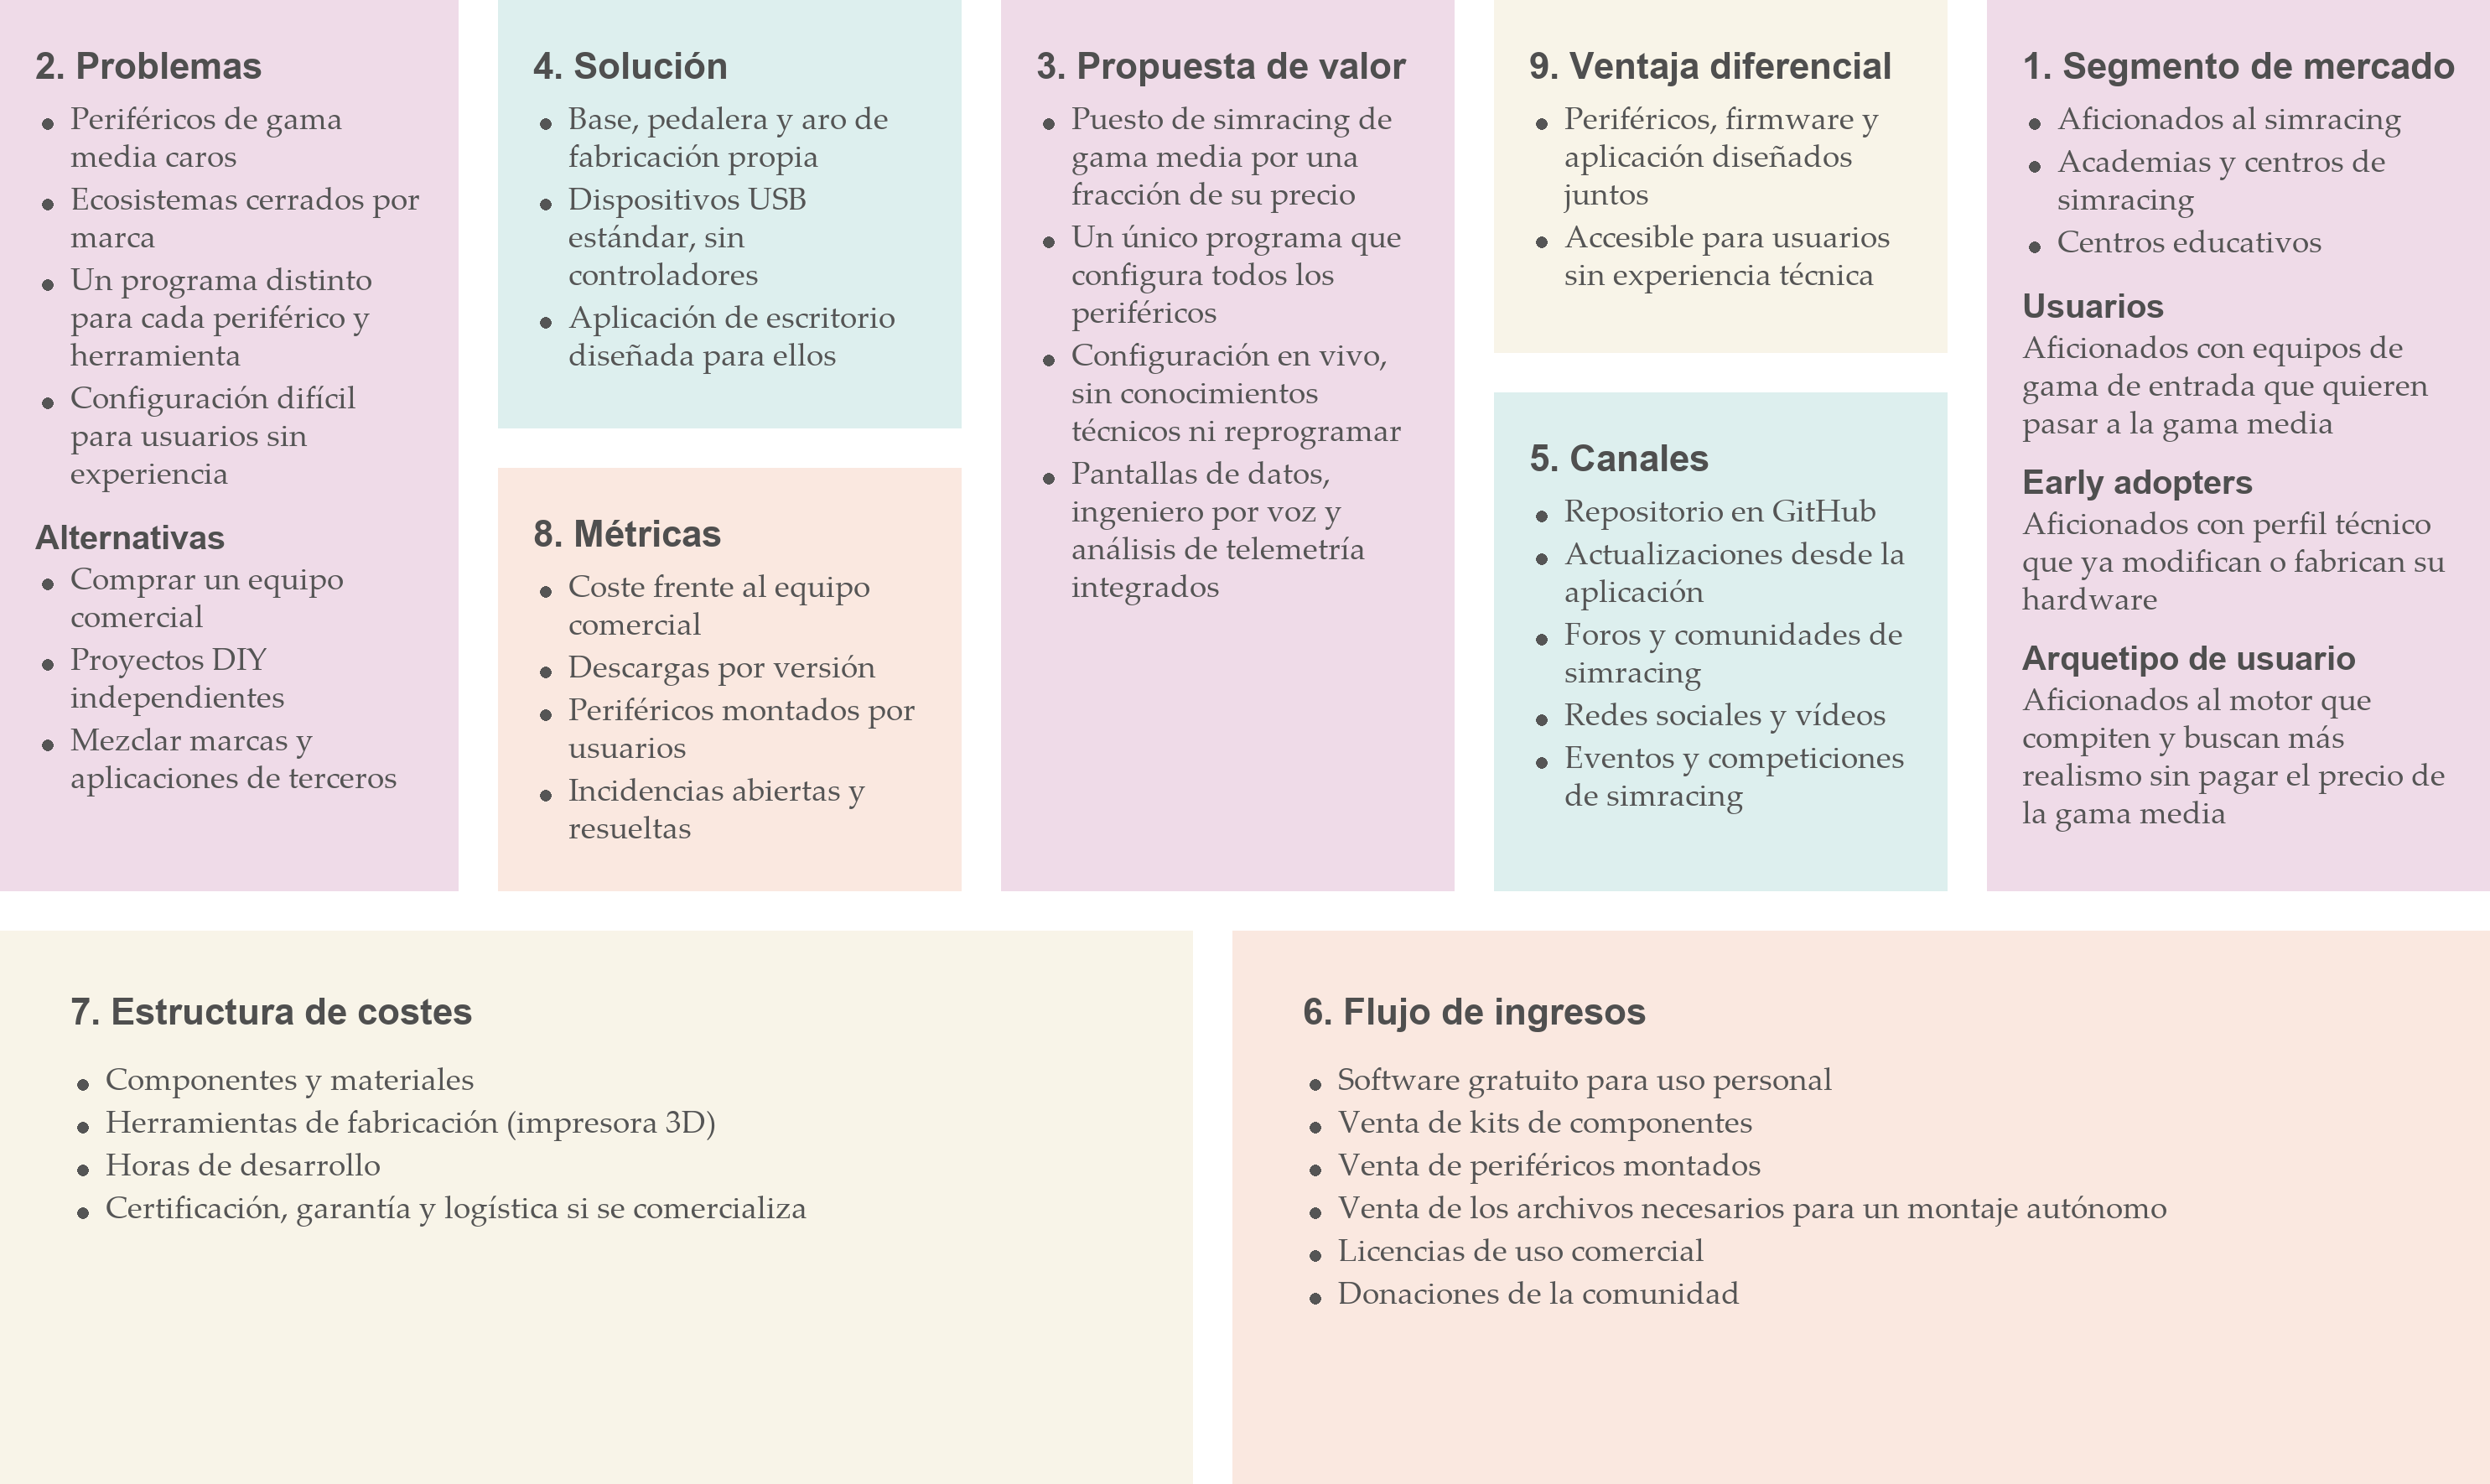
\includegraphics[width=0.9\linewidth, height=0.88\textheight, keepaspectratio]{img/Lean-Canvas.png}
			\caption[Lean Canvas del ecosistema VH SimGrid]{Lean Canvas del ecosistema VH SimGrid. (Fuente propia)}
			\label{fig:lean-canvas}
		\end{figure}
	\end{landscape}
}

\paragraph{Problema y segmentos de clientes.}
El segmento de mercado al que se dirige la propuesta está formado por tres grupos: los aficionados al simracing, las academias y centros de simracing y los centros educativos. Dentro de él, los usuarios principales son los aficionados que ya disponen de un equipo de gama de entrada y quieren dar el salto a la gama media, mientras que los primeros usuarios (\textit{early adopters}) serán los aficionados con perfil técnico que ya modifican o fabrican su propio hardware, dispuestos a montar un periférico si el resultado compensa el esfuerzo. El arquetipo de usuario es el de un aficionado al motor que compite en simuladores y busca más realismo sin pagar el precio de la gama media. 
Los problemas que comparten estos usuarios son los descritos en la sección~\ref{sec:contexto}: los periféricos de gama media son caros, cada fabricante encierra al usuario en su propio ecosistema, cada periférico y cada herramienta de apoyo requiere su propio programa, y configurar el conjunto resulta difícil para quien no tiene experiencia. Hoy existen tres alternativas para resolverlos, que son aquellas con las que compite la propuesta: comprar un equipo comercial y asumir su precio, construir los periféricos a partir de proyectos de fabricación propia independientes entre sí, o combinar periféricos de distintas marcas con varias aplicaciones de terceros.

\paragraph{Propuesta de valor y solución.}
La propuesta de valor de VH SimGrid es ofrecer un puesto de simracing de gama media por una fracción de su precio, configurado desde un único programa que gestiona todos los periféricos. Esa configuración se hará en vivo, sin conocimientos técnicos y sin necesidad de reprogramar los dispositivos, y el mismo programa integrará las pantallas de datos, el ingeniero de pista por voz y el análisis de telemetría que hoy obligan a combinar varias aplicaciones. La solución que materializa esta propuesta es el ecosistema descrito en la sección~\ref{sec:propuesta}: una base, una pedalera y un aro de fabricación propia que funcionan como dispositivos USB estándar, sin controladores, y una aplicación de escritorio diseñada específicamente para ellos.

\paragraph{Canales, fuentes de ingresos y estructura de costes.}
El canal principal de distribución será un repositorio público en GitHub, desde el que se publicarán el instalador de la aplicación y los firmwares de cada versión, y la propia aplicación avisará de las actualizaciones al usuario. Para dar a conocer el proyecto se emplearán los canales en los que se concentra la comunidad: foros y comunidades de simracing, redes sociales y plataformas de vídeo, en las que mostrar los periféricos en funcionamiento es la forma más eficaz de llegar al público, y eventos y competiciones de simracing. 
En cuanto al flujo de ingresos, el software se distribuirá de forma gratuita para uso personal, lo que permite construir una base de usuarios sobre la que apoyar el resto de fuentes: la venta de kits de componentes, la venta de periféricos ya montados para quien no quiera fabricarlos, la venta de los archivos necesarios para que el usuario realice un montaje autónomo, como los modelos para impresión 3D, las licencias de uso comercial para academias y centros de simracing y las donaciones de la comunidad. 
La estructura de costes, al no existir una empresa ni una plantilla, se reduce a los componentes y materiales, las herramientas de fabricación, principalmente la impresora 3D, y las horas de desarrollo, que son con diferencia el coste principal y se {\color{blue}estiman} en la sección~\ref{sec:viabilidad-economica}. Una eventual comercialización añadiría los costes de certificación, garantía y logística.

\paragraph{Métricas clave y ventaja diferencial.}
Las métricas que permitirán comprobar si la propuesta funciona son cuatro. La primera es el coste de un puesto completo frente al de un equipo comercial equivalente, que mide directamente el cumplimiento de la propuesta de valor. Las otras tres miden la adopción y la calidad del sistema una vez publicado: el número de descargas de cada versión, el número de periféricos montados por otros usuarios y las incidencias abiertas y resueltas en el repositorio. Como la aplicación procesa todos los datos en local y no envía información fuera del equipo, estas métricas se obtendrán de los canales públicos y no del uso de la aplicación. Por último, la ventaja diferencial del proyecto es que los periféricos, su firmware y la aplicación se diseñan juntos, una integración que no ofrecen los fabricantes comerciales, sin incentivos para abrir sus ecosistemas a periféricos ajenos, ni los proyectos de fabricación propia, centrados en un único periférico. A ello se suma que el sistema es accesible para usuarios sin experiencia técnica, lo que amplía su público más allá de los aficionados a la electrónica.

\subsection{Análisis de riesgos}
\label{sec:riesgos}

Todo proyecto está expuesto a sucesos que, si se producen, pueden retrasarlo, encarecerlo o impedir que alcance sus objetivos. El análisis de riesgos consiste en identificar esos sucesos antes de que ocurran, estimar su probabilidad y su impacto, y prever las medidas que los evitan o reducen sus consecuencias. En este proyecto los riesgos se agrupan en tres categorías: técnicos, de planificación y coste, y legales. Para cada uno se estima la probabilidad de que ocurra y el impacto que tendría sobre el proyecto en una escala de tres niveles (baja, media y alta), y la combinación de ambas determina su nivel de riesgo y la prioridad con la que debe atenderse{\color{blue}, según los criterios que se definen a continuación}.

{\color{blue}
	\paragraph{Escalas de valoración.}
	Para que la valoración de cada riesgo no dependa de una impresión subjetiva, cada nivel de la escala se asocia a un criterio concreto, recogido en la tabla~\ref{tab:escalas-riesgo}. La probabilidad se expresa por la frecuencia con la que se espera que el suceso se presente durante el desarrollo, que se prevé de unos seis meses. El impacto se mide por sus consecuencias sobre el plazo, el coste, los objetivos del proyecto y, en los casos más graves, la integridad física del usuario o la situación legal del proyecto. Basta con que se cumpla uno de los criterios de impacto para asignar ese nivel.
	
	\begin{table}[htbp]
		\centering
		\caption{Criterios de las escalas de probabilidad e impacto.}
		\label{tab:escalas-riesgo}
		\small
		\begin{tabularx}{\textwidth}{@{}l>{\raggedright\arraybackslash}p{1.4cm}X@{}}
			\toprule
			\textbf{Escala} & \textbf{Nivel} & \textbf{Criterio} \\
			\midrule
			Probabilidad & Baja &
			Poco probable. Si ocurre, se espera como mucho una vez en todo el proyecto (del orden de una vez al año). \\
			& Media &
			Puede ocurrir varias veces a lo largo del proyecto, del orden de una vez al mes. \\
			& Alta &
			Ocurrirá casi con seguridad y de forma recurrente, del orden de una vez a la semana durante las fases afectadas. \\
			\midrule
			Impacto & Bajo &
			Retraso inferior a una semana o sobrecoste inferior a 50~€. No compromete ningún objetivo. \\
			& Medio &
			Retraso de una a cuatro semanas, sobrecoste de 50 a 200~€, u obliga a recortar o aplazar una función secundaria. \\
			& Alto &
			Retraso superior a un mes, sobrecoste superior a 200~€, impide cumplir un objetivo principal, pone en riesgo la integridad física del usuario o tiene consecuencias legales. \\
			\bottomrule
		\end{tabularx}
	\end{table}
	
	El nivel de riesgo se obtiene combinando ambas escalas mediante una matriz de probabilidad e impacto. A cada nivel se le asigna un valor (1 para bajo, 2 para medio y 3 para alto) y el nivel de riesgo resulta del producto de los dos valores, como muestra la tabla~\ref{tab:matriz-riesgo}. Un producto de 1 o 2 corresponde a un riesgo bajo; de 3 o 4, a un riesgo medio, y de 6 o 9, a un riesgo alto.
	
	\begin{table}[htbp]
		\centering
		\caption{Matriz de probabilidad e impacto para obtener el nivel de riesgo.}
		\label{tab:matriz-riesgo}
		\small
		\begin{tabular}{@{}lccc@{}}
			\toprule
			\textbf{Probabilidad} $\backslash$ \textbf{Impacto} & \textbf{Bajo (1)} & \textbf{Medio (2)} & \textbf{Alto (3)} \\
			\midrule
			\textbf{Alta (3)}  & Medio (3) & Alto (6)  & Alto (9) \\
			\textbf{Media (2)} & Bajo (2)  & Medio (4) & Alto (6) \\
			\textbf{Baja (1)}  & Bajo (1)  & Bajo (2)  & Medio (3) \\
			\bottomrule
		\end{tabular}
	\end{table}
	
	El nivel de riesgo fija la prioridad y el tratamiento de cada uno:
	
	\begin{itemize}
		\item \textbf{Bajo}: el riesgo se acepta. No se toman medidas específicas, pero se vigila por si cambia su valoración.
		\item \textbf{Medio}: se planifican medidas preventivas y se revisa su estado al final de cada iteración del desarrollo.
		\item \textbf{Alto}: es prioritario. Las medidas se aplican desde el inicio del proyecto o, como tarde, antes de empezar la fase a la que afecta, y su seguimiento es continuo. No se da por cerrada esa fase mientras el riesgo no se haya reducido.
	\end{itemize}
}

\paragraph{Riesgos técnicos.}
El riesgo más grave del proyecto es la seguridad de la base. Un motor capaz de mover el volante con fuerza puede lesionar las manos o las muñecas del piloto si el firmware falla, si el simulador envía una consigna anómala o si el volante se suelta durante un choque virtual. Además, un error de control puede hacer que el motor oscile o se embale, y una corriente excesiva puede sobrecalentarlo o dañar la controladora y la fuente de alimentación. Su probabilidad es media, porque el desarrollo del firmware implica necesariamente pruebas con el motor en funcionamiento, pero su impacto es alto, ya que afecta a la integridad física del usuario. El segundo riesgo técnico es la disponibilidad de los componentes. El proyecto depende de piezas de bajo coste, como los motores de recambio o las controladoras derivadas de proyectos abiertos, que se fabrican sin un compromiso de continuidad y cuyo precio puede variar, de modo que un componente puede dejar de fabricarse o cambiar de especificaciones durante el desarrollo. El tercer riesgo es la compatibilidad con los simuladores. Cada simulador publica su telemetría en un formato propio, puede cambiarlo con una actualización e interpreta el \textit{force feedback} a su manera, por lo que un periférico que funciona correctamente en un simulador puede comportarse de forma distinta en otro.

\paragraph{Riesgos de planificación y de coste.}
El proyecto abarca diseño mecánico, electrónica, firmware y una aplicación de escritorio, y lo desarrolla una sola persona. El principal riesgo de planificación es, por tanto, que el alcance supere el tiempo disponible, bien porque alguna parte resulte más compleja de lo previsto, como el control del motor o la lectura de la telemetría de cada simulador, bien porque surjan problemas difíciles de diagnosticar al combinar hardware y software. A ello se suma la dependencia de una única persona, que convierte cualquier imprevisto personal en un retraso de todo el proyecto. En cuanto al coste, el riesgo es que el presupuesto de la sección~\ref{sec:viabilidad-economica} se supere por la rotura de componentes durante las pruebas, especialmente en la electrónica de potencia de la base, por la necesidad de repetir piezas impresas en sucesivas iteraciones del diseño o por variaciones en el precio de los componentes.

\paragraph{Riesgos legales: marcas y diseños de referencia.}
El aro toma como referencia el volante de un monoplaza real de Fórmula~1, cuya forma, logotipos y nombres están protegidos por derechos de propiedad industrial e intelectual de sus titulares. Reproducir esos elementos, o usar marcas de terceros para identificar o promocionar el proyecto, podría vulnerar esos derechos, especialmente si el proyecto llegara a comercializarse. Un riesgo similar afecta al software: la aplicación incorporará bibliotecas y componentes de terceros cuyas licencias imponen condiciones de uso y de atribución, y los diseños de pantallas de datos inspirados en coches reales pueden incluir elementos protegidos. Por último, una eventual venta de periféricos obligaría a cumplir la normativa de seguridad de productos eléctricos, cuyo incumplimiento tendría consecuencias legales para el fabricante.

\paragraph{Plan de mitigación.}
La tabla~\ref{tab:riesgos} resume los riesgos identificados, su valoración {\color{blue}según los criterios de las tablas~\ref{tab:escalas-riesgo} y~\ref{tab:matriz-riesgo}} y las medidas previstas para cada uno. La prioridad máxima corresponde a la seguridad de la base, que se aborda como un requisito de diseño: el firmware limitará el par y la velocidad, vigilará la temperatura, frenará el volante al final de su recorrido y cortará el par ante cualquier fallo de comunicación, y estas protecciones se probarán en situaciones límite antes de usar la base con normalidad. Frente a la dependencia de componentes, se elegirán piezas basadas en estándares y con alternativas equivalentes, y se diseñará el firmware de forma que su sustitución afecte lo menos posible al resto del sistema. Frente a la variedad de simuladores, la aplicación aislará la lectura de cada uno en una capa común, de modo que un cambio en un simulador solo afecte a su adaptador. Los riesgos de planificación se reducen con un desarrollo iterativo e incremental, en el que cada periférico se lleva primero a una versión funcional antes de añadir funciones, y con un control de versiones que permita volver a un estado estable. Por último, los riesgos legales se evitan no reproduciendo logotipos ni marcas en las piezas, presentando el aro como un diseño propio inspirado en una referencia y respetando las licencias del software de terceros, cuyos avisos se incluirán con la aplicación.

\begin{table}[htbp]
	\centering
	\caption[Riesgos del proyecto, valoración y medidas de mitigación.]{Riesgos del proyecto, valoración y medidas de mitigación. RT: riesgos técnicos; RP: de planificación y coste; RL: legales.}
	\label{tab:riesgos}
	\small
	\begin{tabularx}{\textwidth}{@{}l>{\raggedright\arraybackslash}p{3.2cm}cccX@{}}
		\toprule
		\textbf{ID} & \textbf{Riesgo} & \textbf{Prob.} & \textbf{Impacto} & \textbf{Nivel} & \textbf{Mitigación} \\
		\midrule
		RT-01 & Seguridad de la base & Media & Alto & Alto &
		Limitar el par y la velocidad, vigilar la temperatura, frenar el volante al final del recorrido y cortar el par ante fallos de comunicación, probándolo en situaciones límite. \\
		RT-02 & Disponibilidad de componentes & Media & Medio & Medio &
		Elegir piezas basadas en estándares y con alternativas equivalentes, y desacoplar el firmware del hardware concreto. \\
		RT-03 & Compatibilidad con los simuladores & Alta & Medio & {\color{blue}Alto} &
		Aislar la lectura de cada simulador en un adaptador sobre una capa común. \\
		RP-01 & Alcance mayor que el tiempo disponible & Alta & Alto & Alto &
		Desarrollo iterativo e incremental: cada periférico llega a una versión funcional antes de ampliarlo. \\
		RP-02 & Dependencia de una sola persona & Media & Alto & Alto &
		Control de versiones y documentación continua para retomar el trabajo desde un estado estable. \\
		RP-03 & Desviación del presupuesto & Media & Medio & Medio &
		Probar la electrónica de potencia de forma progresiva e iterar los prototipos en PLA antes de la pieza final. \\
		RL-01 & Propiedad industrial e intelectual & Media & Alto & Alto &
		No reproducir logotipos ni marcas y presentar el aro como un diseño propio inspirado en una referencia. \\
		RL-02 & Licencias del software de terceros & Baja & Medio & Bajo &
		Revisar las licencias e incluir sus avisos con la aplicación. \\
		RL-03 & Normativa de productos eléctricos & Baja & Alto & Medio &
		Cumplirla antes de una eventual comercialización. \\
		\bottomrule
	\end{tabularx}
\end{table}

\subsection{Viabilidad económica}
\label{sec:viabilidad-economica}

La viabilidad económica se valora desde dos puntos de vista. El primero es el coste de construir un equipo completo, que es el que paga el usuario {\color{blue}y que debe quedar claramente por debajo del de un equipo comercial}. El segundo es el coste total del proyecto, que incluye además el tiempo de desarrollo y los medios empleados. Todas las cifras de esta sección son estimaciones previas al desarrollo.

\paragraph{Presupuesto del proyecto.}
{\color{blue}Para los materiales de los tres periféricos se prevé una inversión de unos 600~euros, asumible con recursos propios y basada en componentes de bajo coste y fácil acceso.} A ese importe hay que sumar los demás conceptos que intervienen en el desarrollo, recogidos en la tabla~\ref{tab:presupuesto}. Se añade una partida de imprevistos del 15~\% sobre los materiales para cubrir los componentes que se dañen durante las pruebas y las piezas que haya que repetir al iterar el diseño. El software empleado es gratuito o dispone de licencia educativa. El concepto de mayor peso es, con diferencia, el tiempo de desarrollo, valorado con el coste horario de un ingeniero junior. Este coste se asume una sola vez, una vez desarrollado el sistema, cada puesto adicional cuesta solo sus materiales.

\begin{table}[htbp]
	\centering
	\caption{Presupuesto estimado del proyecto.}
	\label{tab:presupuesto}
	\small
	\begin{tabular}{|p{0.62\textwidth}|r|}
		\hline
		\textbf{Concepto} & \textbf{Importe (€)} \\
		\hline
		{\color{blue}Materiales de los tres periféricos (estimación)} & {\color{blue}600} \\
		Imprevistos: roturas y repetición de piezas (15~\% de los materiales) & {\color{blue}90} \\
		Software (licencias gratuitas y educativas) & 0 \\
		Desarrollo: 450~h a 25~€/h & 11\,250 \\
		\hline
		\textbf{Total} & {\color{blue}\textbf{11\,940}} \\
		\hline
	\end{tabular}
\end{table}

{\color{blue}Con una inversión en materiales asumible y la mano de obra disponible, el proyecto se considera viable desde el punto de vista económico. La comparación del coste real del equipo terminado con los equipos comerciales se realizará en el capítulo de resultados.}
